\begin{figure}[H]
	\begin{subfigure}{0.5\textwidth}
		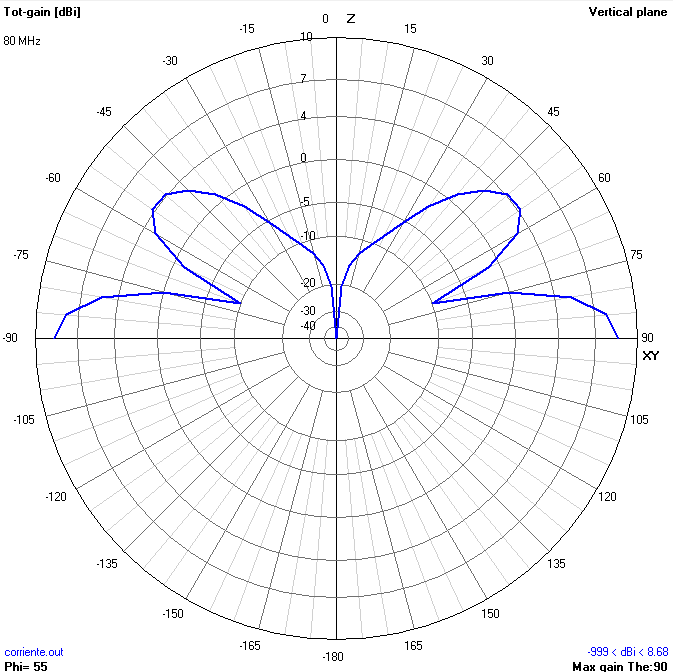
\includegraphics[scale=0.43]{imagenes/2D_80MHz_tierra.png}
	\end{subfigure}	
	\quad
	\begin{subfigure}{0.5\textwidth}
		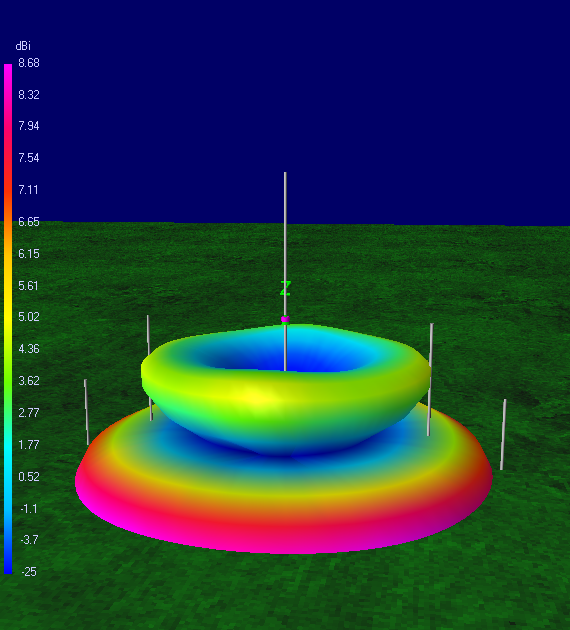
\includegraphics[scale=0.43]{imagenes/3D_80MHz_tierra.png}
	\end{subfigure}
	\caption{$f=\SI{80}{\mega\hertz}$}
	\label{fig.radiacion_80M_tierra}
\end{figure}

\begin{figure}[H]
	\begin{subfigure}{0.5\textwidth}
		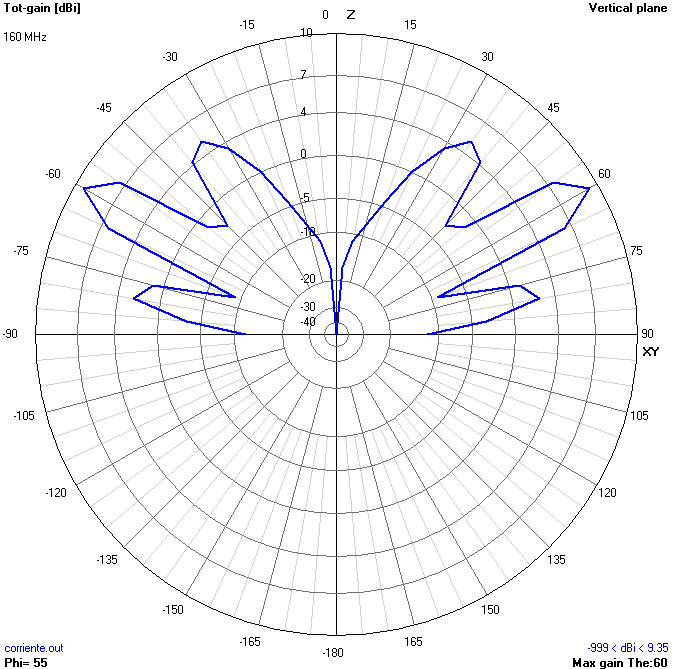
\includegraphics[scale=0.43]{imagenes/2D_160MHz_tierra.png}
	\end{subfigure}	
	\quad
	\begin{subfigure}{0.5\textwidth}
		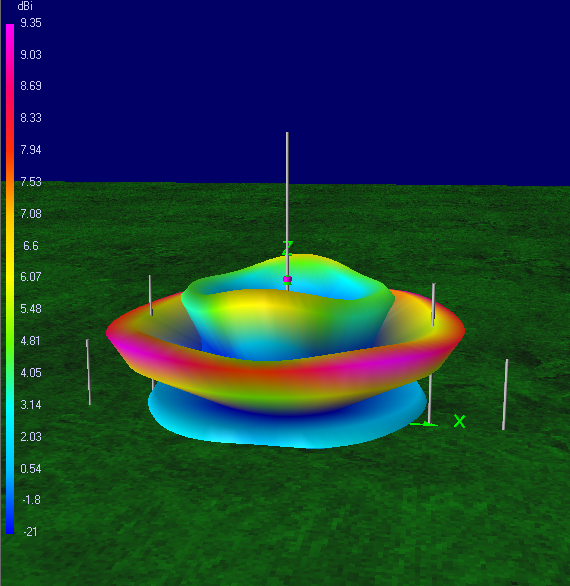
\includegraphics[scale=0.43]{imagenes/3D_160MHz_tierra.png}
	\end{subfigure}
	\caption{$f=\SI{160}{\mega\hertz}$}
	\label{fig.radiacion_160M_tierra}
\end{figure}

\begin{figure}[H]
	\begin{subfigure}{0.5\textwidth}
		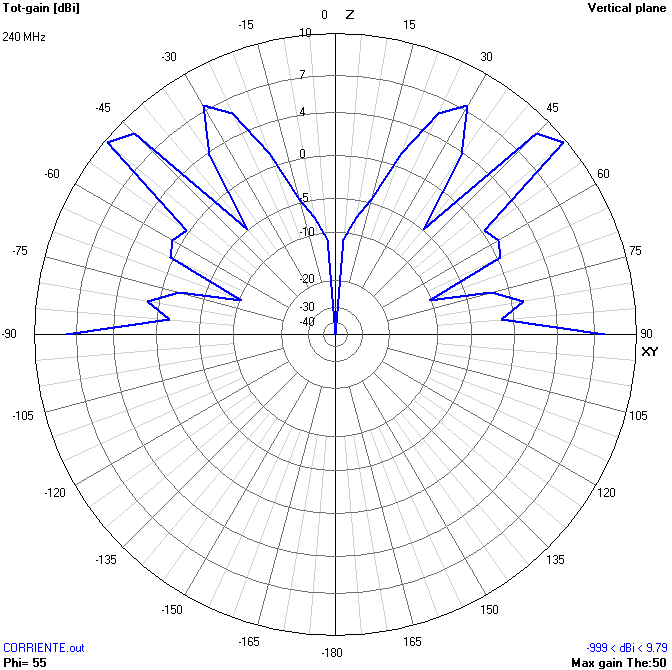
\includegraphics[scale=0.43]{imagenes/2D_240MHz_tierra.png}
	\end{subfigure}	
	\quad
	\begin{subfigure}{0.5\textwidth}
		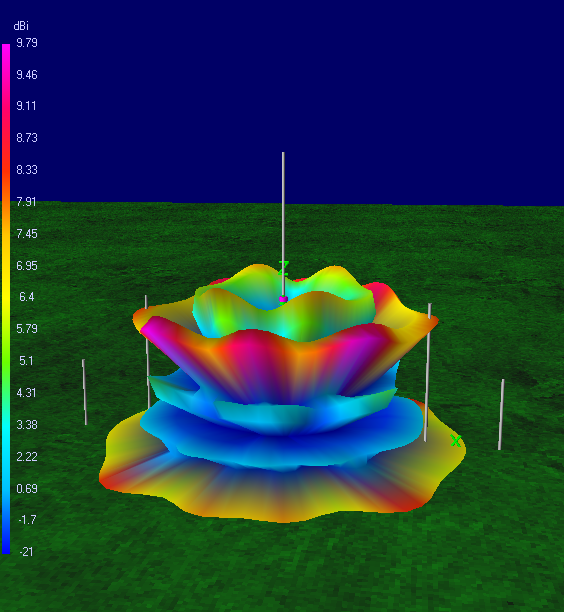
\includegraphics[scale=0.43]{imagenes/3D_240MHz_tierra.png}
	\end{subfigure}
	\caption{$f=\SI{240}{\mega\hertz}$}
	\label{fig.radiacion_240M_tierra}
\end{figure}

\begin{figure}[H]
	\begin{subfigure}{0.5\textwidth}
		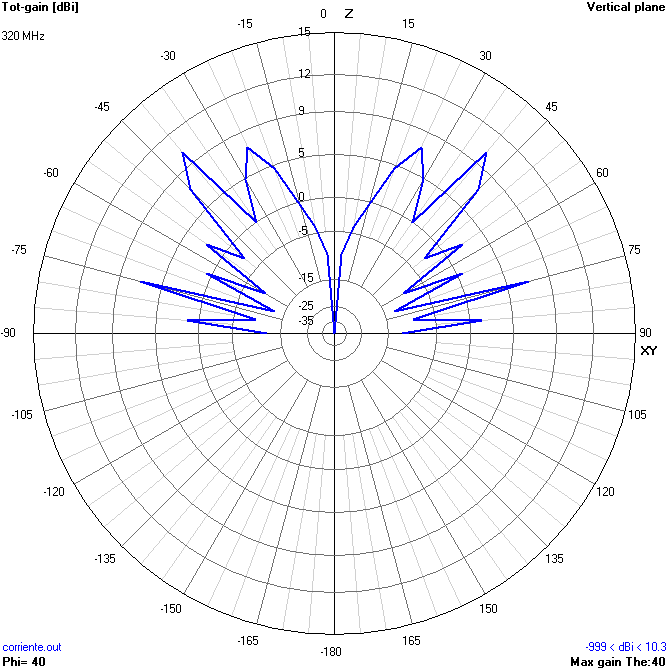
\includegraphics[scale=0.43]{imagenes/2D_320MHz_tierra.png}
	\end{subfigure}	
	\quad
	\begin{subfigure}{0.5\textwidth}
		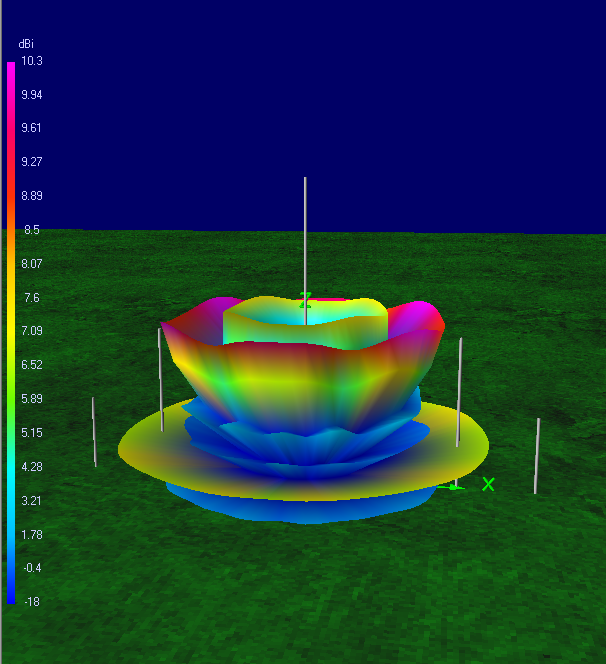
\includegraphics[scale=0.43]{imagenes/3D_320MHz_tierra.png}
	\end{subfigure}
	\caption{$f=\SI{320}{\mega\hertz}$.}
	\label{fig.radiacion_320M_tierra}
\end{figure}

\begin{figure}[H]
	\begin{subfigure}{0.5\textwidth}
		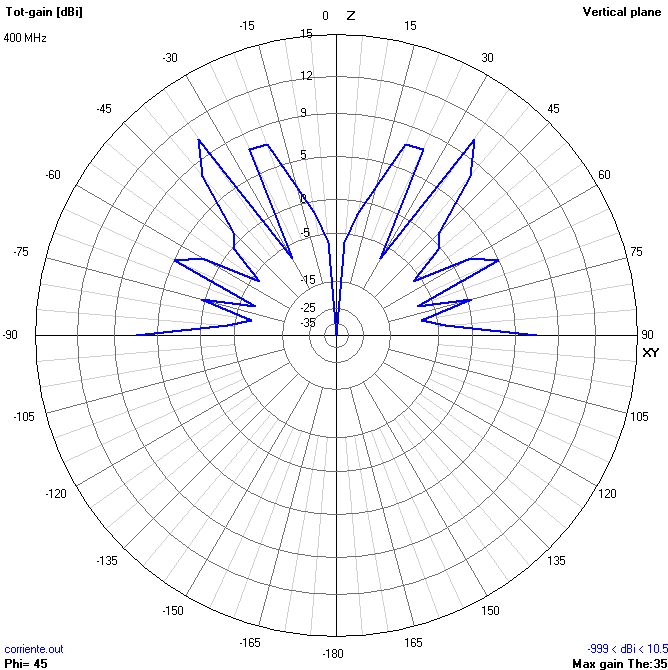
\includegraphics[scale=0.43]{imagenes/2D_400MHz_tierra.png}
	\end{subfigure}	
	\quad
	\begin{subfigure}{0.5\textwidth}
		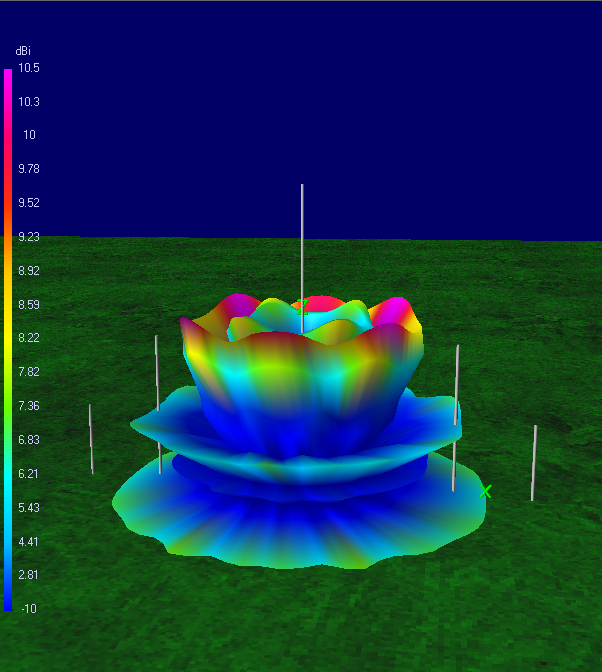
\includegraphics[scale=0.43]{imagenes/3D_400MHz_tierra.png}
	\end{subfigure}
	\caption{$f=\SI{400}{\mega\hertz}$.}
	\label{fig.radiacion_400M_tierra}
\end{figure}

\begin{figure}[H]
	\begin{subfigure}{0.5\textwidth}
		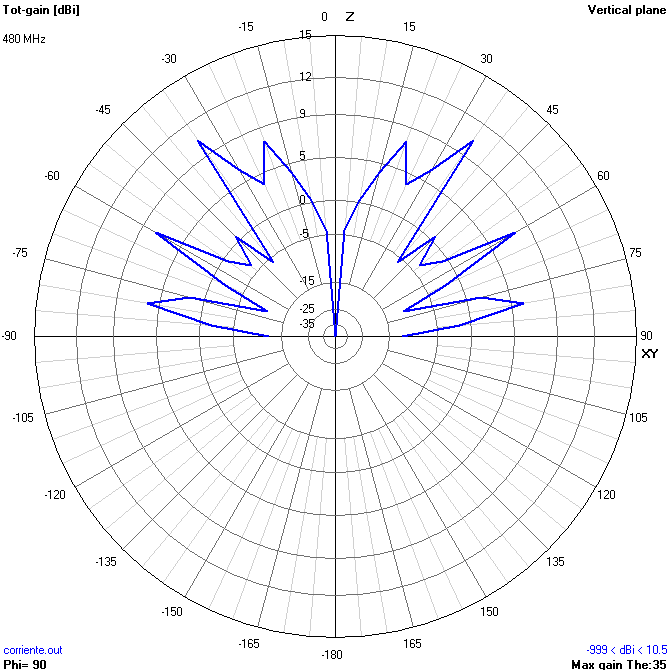
\includegraphics[scale=0.43]{imagenes/2D_480MHz_tierra.png}
	\end{subfigure}	
	\quad
	\begin{subfigure}{0.5\textwidth}
		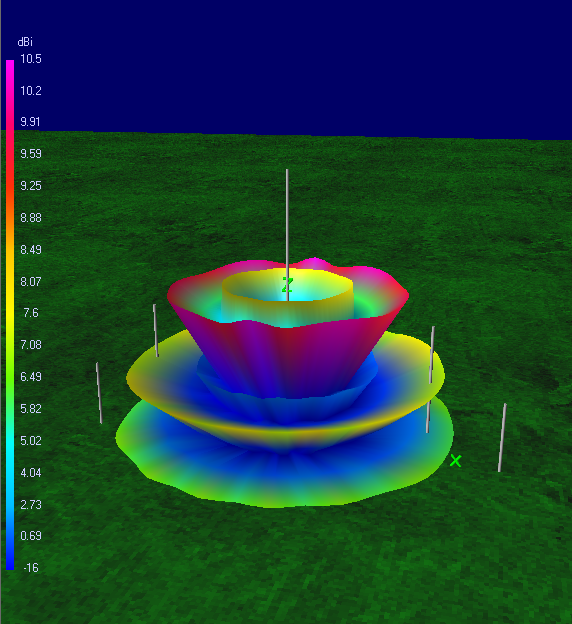
\includegraphics[scale=0.43]{imagenes/3D_480MHz_tierra.png}
	\end{subfigure}
	\caption{$f=\SI{480}{\mega\hertz}$.}
	\label{fig.radiacion_480M_tierra}
\end{figure}	


\begin{table} [H]
	\centering
	\begin{tabular}{ccccccccc}
		\toprule
		& $f [\SI{}{\mega\hertz}]$ 					&  80  & 160  &  240 &  320 &  400 &  480 \\
		\midrule
		\multirow{4}{*}{Espacio libre} & RDF [dB] 	& 7,17 & 5,06 & 6    & 5,69 & 6,3  & 6,36 \\ 
				\cline{2-8}
				& Ángulo ganancia max. 				& 85   & 120  & 135  & 140  & 145  & 150  \\ 
				\cline{2-8}
				& $\#$ lóbulos principales 			& 2    & 8    & 8    & 8    & 8    & 8 \\  
				\cline{2-8}
				& $\#$ lóbulos secundarios 			& 0    & 0    & 2    & 4    & 6    & 8\\
				\midrule		
		\multirow{4}{*}{Plano de tierra} & RDF [dB] & 8,68 & 9,35 & 9,79 & 10,3 & 10,5 & 10,5 \\
				\cline{2-8}
				& Ángulo de ganancia max.			& 90   & 60  & 50  & 40  & 35  & 35 \\
				\cline{2-8}
				& $\#$ lóbulos principales 			& 2    & 4   & 4   & 4   & 4   & 4 \\
				\cline{2-8}
				& $\#$ lóbulos secundarios 			& 2    & 4   & 4   & 8   & 8   & 8 \\
		\bottomrule
	\end{tabular}
	\caption{Resultados.}
	\label{tab.resultados}
\end{table}


En la tabla \ref{tab.resultados} se resumen algunas características relevantes para los casos con y sin plano de tierra. El parámetro $RDF$ representa la diferencia entre la máxima ganancia posible y la ganancia promedio de la antena. Una antena no crea energía, sino que concentra energía en cierta dirección con respecto a otras. Por lo que la ganancia de una antena se refiere a la cantidad de energía radiada en cierta dirección en comparación con la energía que podría radiar una antena isotrópica en la misma dirección con la misma alimentación.
Al agregar el plano a tierra se incrementa la cantidad de lóbulos secundarios (con respecto al caso de espacio libre) y a medida que aumenta la frecuencia la diferencia de ganancia entre los lóbulos secundarios y principales es cada vez menor. También la radiación tiende a concentrarse en el eje $z$ para altas frecuencias, pero a diferencia del caso el espacio libre, con menor ángulo ante una misma frecuencia.
en todos los casos (de espacio libre y con plano a tierra) se obtuvo una eficiencia de aproximadamente 100\%, aunque la presencia de lóbulos secundarios provoca la disminución de dicho parámetro.




